\documentclass{article}
\usepackage{makeidx}
\usepackage{hyperref}
\usepackage{amsmath}
\usepackage{amssymb}
\usepackage{xcolor}
\usepackage{graphicx}

\title{Deep Learning Notes}
\author{Haotian Chen}
\date{}

\makeatletter
\renewcommand\paragraph{\@startsection{paragraph}{4}{\z@}%
                                     {-3.25ex\@plus -1ex \@minus -.2ex}%
                                     {1.5ex \@plus .2ex}%
                                     {\normalfont\normalsize\bfseries}}
\makeatletter

\hypersetup{
    colorlinks=true,
    linkcolor=blue,
    urlcolor=cyan,
}

\setcounter{tocdepth}{4}
\setcounter{secnumdepth}{4}

\makeindex



\begin{document}

\maketitle

\clearpage

\tableofcontents{}

\clearpage

\section{Neural Networks and Deep Learning}

\subsection{Activation Function}

\noindent \textbf{binary step:}

\begin{center}
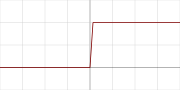
\includegraphics[scale=0.8]{./images/binary_step.png}
\end{center}

\[f(x) = \begin{cases}0&{\text{if }}x<0\\1&{\text{if }}x\geq 0\end{cases}, f(x) \in \{0, 1\}\]
\[f'(x) = \begin{cases}0&{\text{if }}x\neq 0\\{\text{undefined}}&{\text{if }}x=0\end{cases}\]

\noindent \textbf{sigmoid function:}

\begin{center}
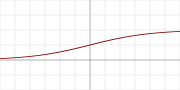
\includegraphics[scale=0.8]{./images/sigmoid.png}
\end{center}

\[f(x) = \sigma (x)={\frac {e^{x}}{e^{x}+1}}={\frac {1}{1+e^{-x}}}, f(x) \in (0, 1)\]
\[f'(x) = f(x)(1-f(x))\]

\noindent \textbf{rectified linear unit: (relu)}

\begin{center}
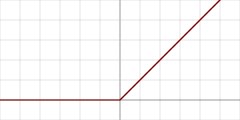
\includegraphics[scale=0.6]{./images/relu.png}
\end{center}

\[f(x) = max\{0, x\} = \begin{cases}0&{\text{if }}x<0\\1&{\text{if }}x\geq 0\end{cases}, f(x) \in [0, +\infty)\]
\[f'(x) = \begin{cases}0&{\text{if }}x<0\\1&{\text{if }}x>0\\{\text{undefined}}&{\text{if }}x=0\end{cases}\]

\subsection{Computation Graphs of Derivatives:}

\begin{center}
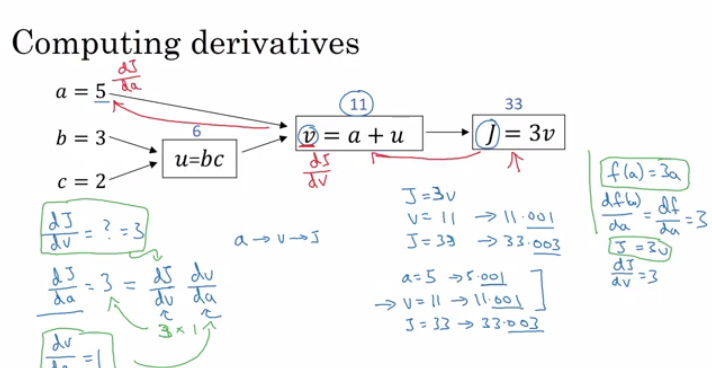
\includegraphics[scale=0.6]{./images/computation_graph.png}
\end{center}

\noindent apply chain rule:

\[\frac{\partial J}{\partial a} = \frac{\partial J}{\partial v} \frac{\partial v}{\partial a} = 3 \times 1 = 3\]

\[\frac{\partial J}{\partial b} = \frac{\partial J}{\partial v} \frac{\partial v}{\partial u} \frac{\partial u}{\partial b} = 3 \times 1 \times 2 = 6\]

\[\frac{\partial J}{\partial c} = \frac{\partial J}{\partial v} \frac{\partial v}{\partial u} \frac{\partial u}{\partial c} = 3 \times 1 \times 3 = 9\]


\subsection{Binary Classification}

Use logistic regression to build a binary classifier.

\begin{center}
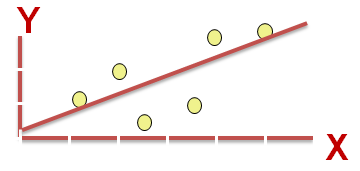
\includegraphics[scale=0.4]{./images/binary_classification.png}
\end{center}

\noindent \textbf{training data:}
\[x \in \mathbb{R}^{n_x}, y \in \{0, 1\}\]
\[\text{\(m\) training examples: } (x^{(i)}, y^{(i)})\:for\:i = 1, \dots, m\]

\[
x^{(i)} = 
\begin{bmatrix}
x^{(i)}_1\\
x^{(i)}_2\\
\vdots\\
x^{(i)}_n
\end{bmatrix}
,
y^{(i)} = y^{(i)}_1
\]

\[X =
\begin{bmatrix}
x^{(1)} & x^{(2)} & \dots & x^{(m)}
\end{bmatrix}
,
Y =
\begin{bmatrix}
y^{(1)} & y^{(2)} & \dots & y^{(m)}
\end{bmatrix}
\]

\[X \in \mathbb{R}^{n_x \times m}, Y \in \mathbb{R}^{1 \times m}\]

\subsection{Logistic Regression}

\noindent Logistic regression is a statistical model that uses a logistic function to model a binary dependent variable.

\bigskip

\noindent Given \(x\), want \(\hat{y} = P(y = 1 | x)\), where \(0 \leq \hat{y} \leq 1\), \(x \in \mathbb{R}^{n_x}\), \(w \in \mathbb{R}^{n_x}\), \(b \in \mathbb{R}\)

\[z = w^Tx + b\]
\[\hat{y} = \sigma(z) = \frac {1}{1+e^{-z}}\]

\[P(y|x) = \begin{cases}\hat{y}&{\text{if }}y = 1\\1 -\hat{y}&{\text{if }}y = 0\end{cases} = \hat{y}^y (1 - \hat{y})^{(1 - y)}\]

\noindent We want to maximize \(P(y|x)\). To make it simpler, because \(log\) function is a strictly increasing function, we can maximize \(log(P(y|x))\) instead.

\[log(P(y|x)) = log(\hat{y}^y (1 - \hat{y})^{(1 - y)}) = ylog(\hat{y}) + (1 - y)log(1 - \hat{y})\]

\noindent Or in reverse, we can minimize \(-log(P(y|x))\), which is called \textbf{loss function}.

\noindent \textbf{loss function: (convex)}

\[L(\hat{y}, y) = -(ylog(\hat{y}) + (1 - y)log(1 - \hat{y}))\]

\noindent \textbf{cost function: (convex)}

\[J(w, b) = \frac{1}{m} \sum^m_{i = 1} L(\hat{y}^{(i)}, y^{(i)}) = - \frac{1}{m} \sum^m_{i = 1} [y^{(i)}log(\hat{y}^{(i)}) + (1 - y^{(i)})log(1 - \hat{y}^{(i)})]\]

\noindent \textbf{gradient descent:} with learning rate \(\alpha\), find best \(w\), \(b\) to minimize \(J(w, b)\)

\noindent repeat until convergence \{
\[w_j =: w_j - \alpha \frac{\partial}{\partial w_j} J(w, b) = w_j - \alpha \frac{1}{m} \sum^m_{i = 1} (\hat{y}^{(i)} - y^{(i)}) x^{(i)}_j\]
\[b =: b - \alpha \frac{\partial}{\partial b} J(w, b) = b - \alpha \frac{1}{m} \sum^m_{i = 1} (\hat{y}^{(i)} - y^{(i)})\]
\centerline{simultaneously update \(w_j\) and \(b\), \(j \in [1, n]\)}
\}

\bigskip

\noindent \textbf{vectorized implementation}:

\noindent repeat until convergence \{
\[w =: w - \alpha \frac{1}{m} X (\sigma(w^TX + b) - Y)^T\]
\[b =: b - \alpha \frac{1}{m} sum\{\sigma(w^TX + b) - Y\}\]
\}

\subsection{Neural Network}

\noindent \textbf{Basic Structure:}

\begin{center}
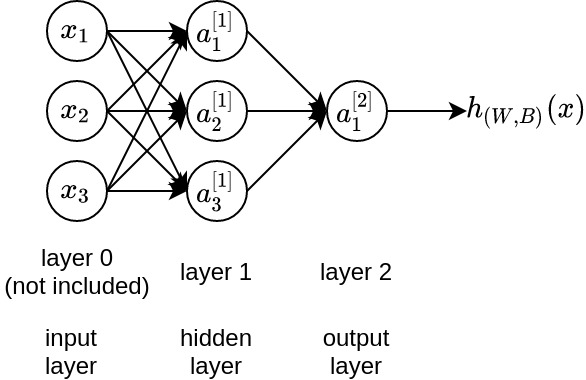
\includegraphics[scale=0.4]{./images/neural_network.jpg}
\end{center}
\[a_i^{[j]} = \text{"activation" of unit i in layer j}\]
\[W^{[j]} = \text{matrix of weights (edges) from layer j to j + 1}\]
\[B^{[j]} = \text{vector of biases (nodes) from layer j to j + 1}\]

\[a_1^{[1]} = \sigma(W_{11}^{[0]} x_1 + W_{12}^{[0]} x_2 + W_{13}^{[0]} x_3 + B_{1}^{[0]})\]
\[a_2^{[1]} = \sigma(W_{21}^{[0]} x_1 + W_{22}^{[0]} x_2 + W_{23}^{[0]} x_3 + B_{2}^{[0]})\]
\[a_3^{[1]} = \sigma(W_{31}^{[0]} x_1 + W_{32}^{[0]} x_2 + W_{33}^{[0]} x_3 + B_{3}^{[0]})\]
\[h_{(W, B)}(x) = a_1^{[2]} = \sigma(W_{11}^{[1]} a_1^{[1]} + W_{12}^{[1]} a_2^{[1]} + W_{13}^{[1]} a_3^{[1]} + B_{1}^{[1]})\]

\bigskip

\noindent If network has \(s_j\) units in layer \(j\), \(s_{j + 1}\) units in layer \(j + 1\), then \(W_j\) will be of dimension \(s_{j + 1} \times s_j\), \(B_j\) will be of dimension \(s_{j + 1} \times 1\).

\bigskip

\noindent \textbf{Generalized Model (one vs all):}

\begin{center}
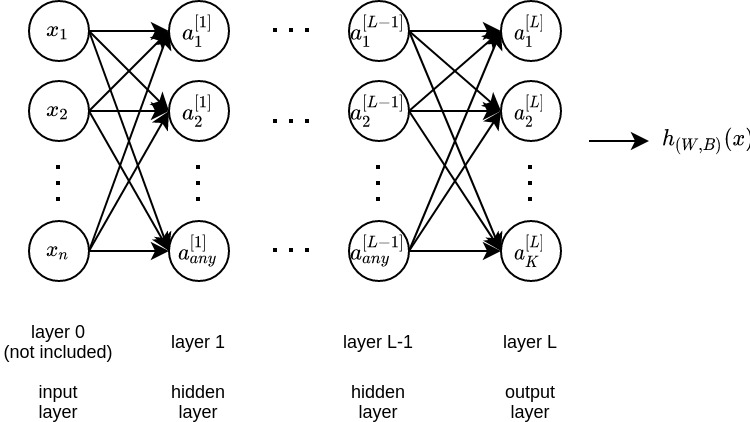
\includegraphics[scale=0.4]{./images/neural_network_generalized.jpg}
\end{center}

\noindent For a neural network that has:

\[L = \text{total number of layers in the network}\]
\[s_l = \text{number of units in layer } l\]
\[K = \text{number of output units/classes}\]

\noindent assume \(a^{[0]} = x, a^{[L]} = h_{(W, B)}(x)\), let:

\[z^{[l]} = W^{[l - 1]} a^{[l - 1]} + B^{[l - 1]}\]
\[a^{[l]} = \sigma(z^{[l]})\]
\[h_{(W, B)}(x) = a^{[L]} = \sigma(z^{[L]})\]

\bigskip

\noindent \textbf{regularized cost function:}
\[J(W, B) = - \frac{1}{m} \sum_{i = 1}^{m} \sum_{k = 1}^{K} [y^{(i)}_k log(h_{(W, B)} (x^{(i)})_k) + (1 - y^{(i)}_k) log(1 - h_{(W, B)}(x^{(i)})_k)] + \frac{\lambda}{2m} \sum_{l = 0}^{L - 1} \sum_{i = 1}^{s_l} \sum_{j = 1}^{s_{l + 1}} (W_{j, i}^{(l)})^{2}\]

\printindex

\end{document}